\section{Usage and Potential Impact Across User Groups}
\label{sec:usage}

This section discusses how SWLS can be used and the expected impact it may have across different user groups.
As a language server, SWLS provides functionality that is independent of specific editors, making it highly versatile.
Some editors, such as NeoVim\footnote{\url{https://neovim.io/}}, treat language servers as first-class citizens, offering seamless integration.
Others, like Visual Studio Code\footnote{\url{https://code.visualstudio.com/}} and Monaco\footnote{\url{https://microsoft.github.io/monaco-editor/}}, require additional glue code to enable effective interaction.
Regardless of the editor, SWLS delivers a consistent set of features that enhance the user experience across all supported platforms.

All code is under a MIT licence available on github\footnote{\url{https://github.com/ajuvercr/semantic-web-lsp}}.
There are currently three ways to interact with SWLS:
\begin{enumerate}
  \item Download the VSCode extension from the market place\footnote{\url{https://marketplace.visualstudio.com/items?itemName=ajuvercr.semantic-web-lsp}}.
  \item Download and compile the binary locally and integrate it into NeoVim\footnote{Installation instruction are available in the README \url{https://github.com/ajuvercr/semantic-web-lsp}}.
  \item Go to the demo available online\footnote{\url{https://ajuvercr.github.io/semantic-web-lsp/}}.
\end{enumerate}

In the demo, users are presented with four distinct editors, each tailored to a specific use case.
A toy ontology and its accompanying SHACL shapes serve as foundational resources for the other editors.
One editor is designed for creating a small dataset based on the toy ontology.
Another editor showcases a simple SPARQL query, which, when executed using a SPARQL client, could provide insights from data structured according to the ontology.
This setup allows users to immerse themselves in different personas, gaining hands-on experience with various aspects of semantic data workflows.

While all editors, except for the SPARQL editor, are functionally the same, 
the visual seperation improves the realism of the tasks at hand.
Below, we discuss how SWLS benefits each user group and validate its utility in practice.
We first go over the key ways the SWLS might help users, then we will apply these ways to the different user groups defined in Section \ref{sec:introduction}, and how those users groups can be assisted by the SWLS.

\subsection{Key Improvements by SWLS}

\begin{figure}[tb]
    \centering
    \begin{subfigure}{0.48\textwidth}
      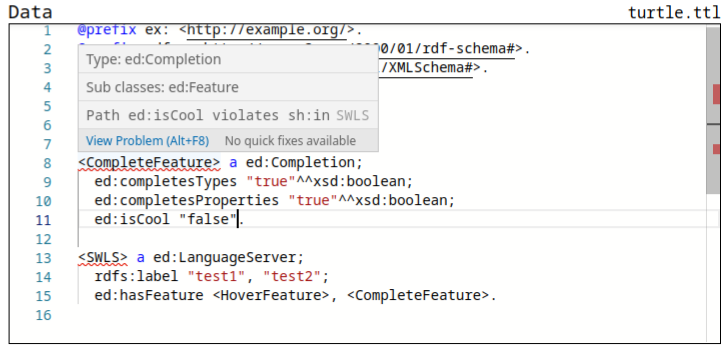
\includegraphics[width=\textwidth]{./images/hover.png}
      \caption{SWLS shows the user type information on hover as well as diagnostics}
      \label{hover}
    \end{subfigure}
    \hfill
    \begin{subfigure}{0.48\textwidth}
      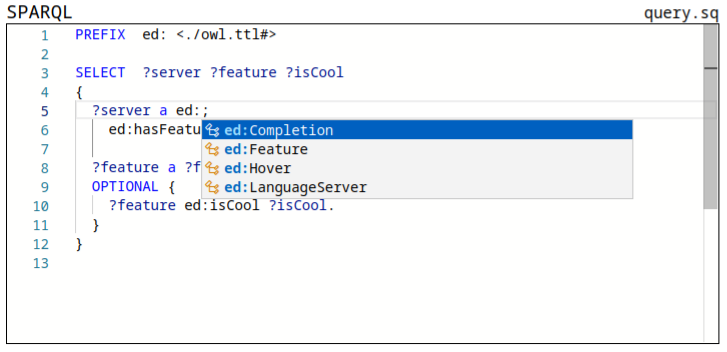
\includegraphics[width=\textwidth]{./images/class.png}
      \caption{SWLS completes a class when the user wants to write a class}
      \label{class_completion}
    \end{subfigure}
    \hfill
    \begin{subfigure}{0.48\textwidth}
      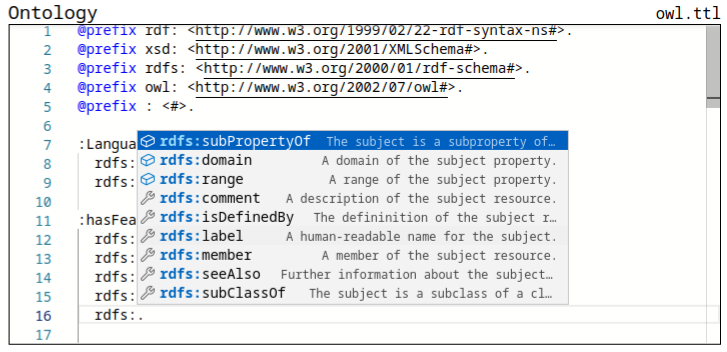
\includegraphics[width=\textwidth]{./images/property.png}
      \caption{SWLS completes properties, first the properties with the correct domain}
      \label{property_completion}
    \end{subfigure}
    \hfill
    \begin{subfigure}{0.48\textwidth}
      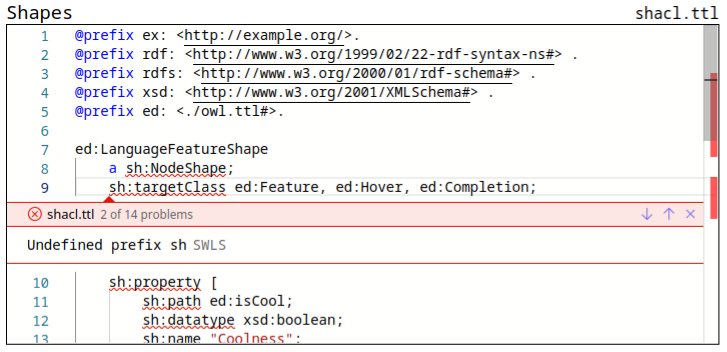
\includegraphics[width=\textwidth]{./images/undefined.png}
      \caption{SWLS notifies the user of undefined prefixes}
      \label{undefined_prefix}
    \end{subfigure}
    \caption{
      Demo application that shows the usage of SWLS. Features include hover information, autocompletion and diagnostics.
    }\label{lst:Demo}
\end{figure}

SWLS enhances development efficiency by providing robust autocompletion capabilities, as illustrated in Figures \ref{class_completion} and \ref{property_completion}.
These features facilitate the creation of semantic documents by accelerating the authoring process and reducing the likelihood of errors.
Whether defining ontologies, constructing SHACL shapes, or formulating SPARQL queries, context-aware suggestions for relevant classes and properties minimize repetitive tasks and cognitive effort, allowing users to concentrate on the conceptual aspects of their work.
Additionally, autocompletion assists users in exploring the current domain by offering informed suggestions based on contextual information.

Beyond efficiency, SWLS enhances comprehension by delivering real-time feedback on semantic data.
It improves users' confidence in both syntax and semantics by identifying issues such as undefined prefixes (Figure \ref{undefined_prefix}) and SHACL constraint violations (Figure \ref{hover}).
The hover feature (Figure \ref{hover}) provides detailed information, including associated classes, enabling users to quickly understand the structure and relationships within a document.
This immediate access to contextual insights and validation mechanisms reduces reliance on external references and serves as an educational aid for mastering Semantic Web technologies.


\subsection{User groups}

\paragraph{Power users,} who frequently interact with Semantic Web technologies, rely on their deep understanding of common properties and domain-specific knowledge to navigate tasks efficiently.
SWLS enhances their workflows by providing robust autocompletion features that streamline document creation and reduce repetitive tasks.
Additionally, the language server supports quality assurance by helping power users identify invalid entities (using shape validation), ensuring their semantic documents are both accurate and high quality.

\paragraph{For newcomers to the Semantic Web,} engaging with these technologies can be daunting due to challenges with syntax, semantics, and validation. 
SWLS addresses these pain points by providing immediate feedback on syntax errors, which helps users learn the correct structure and lessens frustration.
The autocompletion feature offers guided support by suggesting relevant properties, allowing users to build confidence in creating semantic documents.
Moreover, validation tools play an educational role: newcomers can intentionally trigger validation errors to understand what constitutes a faulty document, turning mistakes into valuable learning opportunities.

\paragraph{Domain experts,} a specialized subset of power users, focus on assessing and curating domain-specific ontologies.
By hovering over properties and classes (Figure \ref{hover}), domain experts can quickly verify descriptions and relationships, ensuring the ontology aligns with their domain knowledge.
Autocompletion further aids in this process by completing relevant terms, helping experts assess whether the ontology feels correct in practice.

\paragraph{Data engineers,} would primarily work with SPARQL queries to extract meaningful insights from semantic data. 
For these users, SWLS provides support by offering autocompletion for classes and properties, as well as syntax validation to prevent errors during query formulation. 
These features significantly enhance productivity by reducing the time spent debugging queries and ensuring accurate results. 
By streamlining the querying process, SWLS enables data engineers to focus on deriving insights rather than resolving technical challenges.


